\section{The connection between extreme events and transitioning systems}

%This changes on the response of the system have implications on the behaviour of noise on the system, which translates to changes in the statistical properties of the distribution of the observables at this transitions.  


We now define several metrics to be applied to bifurcations in deterministic systems in the presence of noise, when external parameters are 'slowly' varying.
%Such metrics are specially useful when extreme events appear during the transit
%Indicators like the sample standard deviation, the autocorrelation, skewness and kurtosis, autocorrelation at lag-1 (AR-1) have been used as EWS\footnote{is it??, ask saulo a cite from paper using this in wave forecast}.

%\jk{A widely used index in that regard is kurtosis, i.e.,the 4th moment of the distribution }
The effect of CSD on the statistical properties of the system has inspired the proposal of a  so-called Pareto metric~\cite{Kasparian_pareto}.


\subsection{Tail related metrics}

The Pareto metric is one of many statistical functions that can be used to estimate  how 'heavy tailed' is a  probability distribution function (PDF). As discussed before, the CSD near the bifurcation of the system implies changes on the statistics of the noise.
In particular, this can give ride to  the appearance or frequency increase of extreme events in the systems close to tipping. 

In the rest of this section we will present a modification to the Pareto metric, and compare this to other tail related metrics used for EWS. We will first discuss this modification, and then construct a toy example of a sharp transition in sampled data, to understand how the metric behaves compared to others. 
Then we will use this metric on a series of systems with additive noise, by integrating  their stochastic differential equations (SDE), and discuss its performance. 

\subsubsection{Relative tail weight}

The Relative tail weight (RTW) metric considered in the present work is a slight generalization of the so-called Pareto metric proposed by \cite{Kasparian_pareto}. 
Given a time series of length $N$, this metric characterizes the weight of the PDF tail by calculating the total weight beyond a given threshold:
\begin{equation}
	M_p(I,k)=\frac{\sum^{k N}_{i=1} I_i}{\sum^{N}_{i=1} I_i}
	\label{eq:Pareto_original}
\end{equation}
%\begin{equation}
%   M(I,k)=\frac{\sum^{N}_{i=(1-k)N} I_i}{\sum^{N}_{i=1} I_i}
%  \label{eq:Pareto_original}
%\end{equation}
where the  individual measurements $I_i$ are sorted by descending order ($I_1\geq I_2\geq .. \geq I_n$) and $k$ defines the fraction of the data points that are attributed to the tail. 
For example, $k=0.2$ means that the metric considers the relative weight of the last $20\%$ of the distribution\footnote{This choice of $k$ was first inspired by the Pareto principle.}. 
This metric was successfully applied to the characterization of the pulse-to-pulse fluctuations of the spectral broadening in ultrashort laser filaments, showing that a long-tailed distribution only occurred on the edges of the self-phase modulation spectrum \citep{Kasparian_pareto}.

Since \cref{eq:Pareto_original} is a direct function of the measurement and not the distribution, whether the measurements take positive or negative values will change the result. 
% The original definition of equation \ref{eq:Pareto_original} depends on the absolute value of the mode, or the average of the probability distribution function (PDF).
Indeed, shifting the whole distribution to high values without deforming it will decrease the $M_p$ value since  measurements outside the $k$ percentile take negative values. 
We therefore adapt a new definition by shifting the distribution so that the minimum data point $I_N$ is set to 0. Therefore,

\begin{equation}
	\mathrm{RTW}_{max}(I,k)=\frac{\sum^{k N}_{i=N} (I_i-I_N)}{\sum^{N}_{i=1} (I_i-I_N)}=\frac{\sum^{k N}_{i=N} I_i-k N I_N}{\sum^{N}_{i=1} I_i-NI_N} 
	\label{eq:pareto_offset}
\end{equation}


%  \begin{equation}
	%     M(I,k)_N=\frac{\sum^{N}_{i=(1-k)N} (I_i-I_0)}{\sum^{N}_{i=1} (I_i-I_0)}=\frac{\sum^{N}_{i=(1-k)N} I_i-k N I_0}{\sum^{N}_{i=1} I_i-NI_0} 
	%    \label{eq:pareto_offset}
	%\end{equation}
	
	\begin{figure}[h]
		\centering
		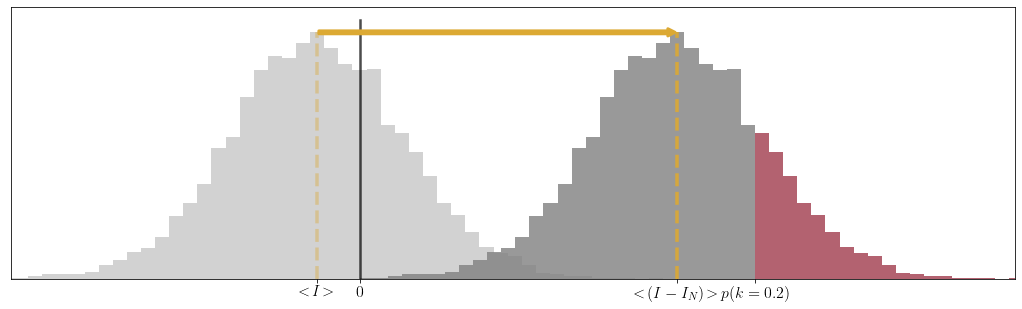
\includegraphics[width=\columnwidth]{Images/Metrics/pareto_shift_explanation.png}
		\caption{Shifting the distribution to have it defined positive, and taking integrating over the highest $k$ percentile (magenta).}
		%	\caption{Events per ms}
		\label{fig:pareto_shift}
	\end{figure}
	
	This adapted $M$ is quite dependent on the value of $I_N$, so that it is mostly adapted to asymmetric distributions where the low-value side cutoff is quite abrupt, so that for $N$ sufficiently large, $I_{min}$ of each data set should converge. 
	
	
	\subsubsection{Extension to consider heavy-tailed distributions on the left side of the PDF}
	
	As discussed above, the definition of $M_p$ in \cref{eq:pareto_offset} focuses on heavy tails on the right side of the PDF (large values). To extend it, we propose to flip the distribution as a whole around its median, then apply the definition in \cref{eq:pareto_offset}. The choice of the median as the flipping axis is consistent with the fact that the Pareto-metric focuses on percentiles. Thus, we consider the flipped intensity distributions:
	
	\begin{equation}
		 \hat{I}_i=2I_{50}-I_i 
	\end{equation}
	and the metric for low values becomes $\mathrm{RTW}_\textrm{low}(I,k)=\mathrm{RTW}_\textrm{max}(\hat{I},k)$
	
	In this way the metric  provides information on the heaviest tail on either side:
	
	\begin{equation}
		\begin{aligned}
		 \mathrm{RTW}(I,k)&=\max(\mathrm{RTW}_\textrm{low}(I,k),\mathrm{RTW}_\textrm{max}(I,k))\\
		 &=\max(\mathrm{RTW}_\textrm{max}(I,k), \mathrm{RTW}_\textrm{max}(\hat{I},k))
		\end{aligned}
	\end{equation}
	
	Here the choice of the $maximum$ of either RTW$_\textrm{max,low}$ is because we want to know what is happening to the more 'extreme' tail, whichever it might be. 
	
	
	Another possible choice is to construct a complex metric RTWc defined as
	
	\begin{equation}
		\mathrm{RTWc}(I,k)=\mathrm{RTW}_\textrm{max}(I,k) + i\, \mathrm{RTW}_\textrm{low}(I,k)
		\label{eq:RTWc}
	\end{equation}
	
	In this case, the absolute value gives information of the intensity of the tail weight in the distribution taking into account both tails, while the angle between $\textrm{RTW}_\textrm{max}$ and $i \textrm{RTW}_\textrm{low} $ encodes information of the asymmetry between the tails.
	
	In this case, for a symmetric distribution the complex metric is related to the one defined by the maximum as 
	
		\begin{equation}
	|\mathrm{RTWc}(I,k)|=\sqrt{\mathrm{RTW}_\textrm{max}^2+\mathrm{RTW}_\textrm{low}^2}=\sqrt{2}\,\mathrm{RTW}_\textrm{max}=\sqrt{2}\,\mathrm{RTW}
		\end{equation}
	
	Thus, the absolute value of RTW is no longer bounded between $(0,1)$ but between $(0,\sqrt{2}$).
	
	
	\subsubsection{Kurtosis and unbiased estimators}
	
	
	The kurtosis of a distribution evaluates the flatness of the PDF mode and the extension of the tails. It is defined as
	\begin{equation}
		\beta_2 = \frac{\sum_{i=1}^N{\left(I_i - <\!I\!>\right)^4}}{\sigma^4}
	\end{equation}
	where $\sigma$ is the standard deviation. While kurtosis is good as a measure of the tails \citep{kurtosisRIP}, some properties like its bias (see below) and heavy dependence on single and large events \citep{KIM200456} mean it might not be the best choice under some circumstances. 
	
	In this work we use the excess kurtosis $\tilde{\beta_2}=\beta_2-3$, defined this way to keep the Gaussian excess kurtosis equal to $0$.
	
	We will show that the use of excess kurtosis for some applications as an indicator for the tail is not practical, and it might be better to use another indicator for real, finite amounts of data. 
	In \cite{Bono_2019,KIM200456} it is recalled that kurtosis can be a biased statistic and two unbiased kurtosis estimators, the Hogg $Hg$ and the Moors $Mo$, are explored:
	
	\begin{equation}        	   
		Hg=\frac{U_{0.05}-L_{0.05}}{U_{0.5}-L_{0.5}}-2.59
		\label{eq: Hogg}
	\end{equation}
	
	\begin{equation}               
		Mo=\frac{(E_7-E_5)+(E_3-E_1)}{E_6-E_2}-1.23
		\label{eq: Moors}
	\end{equation}
	
	where $U_{m}$ and $L_{m}$ refer to the mean of the Upper and Lower $m$ quantiles, respectively. This means that $U_{m}=\frac{1}{m}\int_{1-m}^1 F^{-1}(y)dy$ and $L_{m}=\frac{1}{m}\int_{0}^m F^{-1}(y)dy$, where $F$ is the cumulative distribution function for ${I_i}$\footnote{\cite{Bono_2019,KIM200456} have  different definitions of the unbiased kurtosis estimators $Kr_2$ and $Kr_3$. \cite{Bono_2019} uses these definitions for the Hogg estimators with $m=0.05$ (\cref{eq: Hogg}) and $m=0.2$ (\cref{eq: Hogg}). While \cite{KIM200456} defines $Kr_2$ as the Moors estimator (\cref{eq: Moors}) and $Kr_3$ as the Hogg estimators with $m=0.05$ (\cref{eq: Hogg}). }.
	 $E_n$ in \cref{eq: Moors} are the respective $n$-th octiles. 
	Both definitions are displaced with respect to their values for a Gaussian distribution to be compared to excess kurtosis.
	
	It should be noted that in \cite{KIM200456} another tail metric by Crow and Siddiqui (page 6) is also explored:
	
	\[
	Kr_{CS}=\frac{F^{-1}(1-\alpha)+F^{-1}(\alpha)}{F^{-1}(1-\beta)-F^{-1}(\beta)}
	\]
	
	with $\alpha = 0.025$ and $\beta= 0.25$. 
	However is it shown that this is not as good compared to $Hg$ and $Mo$, and thus will not be considered in this work.
		
	\subsection{Common values}
	
	These metrics share a basic property. They take constant values for some distributions of given shape, like the uniform distribution, the Gaussian distribution, the Rayleigh distribution and the exponential distribution (Table \ref{table: constant shape}).
	
	\begin{table}[h]
		\centering
		\caption{ \label{tab:indicescte} Metric values for typical distributions.}
		\begin{tabular}{| l | l | l | l  |l | l |}
			\hline
			Distribution & RTW & $\left| \mathrm{RTWc}\right| $  & Excess kurtosis  & Hg & Mo\\
			\hline
			Uniform & 0.36 & 0.5 & -1.2  & -0.69 & -0.24 \\
			Gaussian& 0.27 & 0.38 & 0 & 0 & 0\\
			Rayleigh & 0.36 & 0.44 & 0.24 & -0.11 & -0.03\\
			Exponential & 0.52 & 0.57 & 6 & 0.28 & 0.56 \\
			\hline
		\end{tabular}
		\label{table: constant shape}
	\end{table}
	
	This means that, no matter which scale parameter is used for these distributions, they have a constant value for all such tail metrics. 
	Thus, we consider to be requirement of any tail metric. \footnote{Maybe a measure of sensitivity for a given statistic $St$ could be $\frac{Abs(St(gaussian)-St(exponential))}{St(gaussian)}$.. though maybe it is better between two values of the same distribution.. like gamma(0.5) and gamma(2).. so this is a slope in a plot St(gamma) vs. gamma. It would be more apples-to-apples comparison. Finding a distribution that changes linearly for some metric would be best(?)
	}
	
	This is not true for distributions like the Weibull, the Gamma or the Lognormal (among others) that change shape as a function of their parameters\footnote{The excess kurtosis of the lognormal is $K=e^{4\sigma^2}+2e^{3\sigma^2}+3e^{2\sigma^2}$-6; for the Gamma function $K=6/\alpha$ .}.
	
	For comparison with \cite{Bono_2019}, we add the table \ref{table: changing shape}.
	
	\begin{table}[h]
		\centering
		\begin{tabular}{| l | l | l | l | l | l |}
			\hline
			Distribution & RTW & $\left| \mathrm{RTWc}\right| $  & Excess kurtosis\footnote{Excess kurtosis for Gamma PDF is $6/\alpha$; for lognormal distribution is $e^{4\sigma^2}+2e^{3\sigma^2}+3e^{2\sigma^2}-6$} & Hg & Mo\\
			\hline
			lognormal($\zeta=1$,$\alpha=0.5$) & 0.39 & 0.44 & 5.9  & 0.28 & 0.06 \\
			Gamma ($\alpha=0.5$)& 0.65 & 0.68 & 12  & 0.68 & 0.25 \\
			Gamma ($\alpha=2$)& 0.43 &0.48 & 3 &  0.12 & 0.03 \\
			Gamma ($\alpha=4$)& 0.36 & 0.43 & 1.5 & 0.06 & 0.21\\
			\hline
		\end{tabular}
			\caption{ Some values for shape dependent distributions. Here $\alpha$ is the shape parameters of the distributions.\label{tab:indices}}
		\label{table: changing shape}
	\end{table}
	
%\url{https://variation.com/wp-content/distribution_analyzer_help/hs128.htm}}
	
	
	
	
	
	%	\begin{center}
		%		\underline{Table of distributions with constant value: \ag{Make this a real table, with a proper legend + label}}
		%		
		%		\begin{minipage}[t]{0.32\textwidth}
			%			Pareto centered $k=0.2$
			%			
			%			\begin{tabular}{ l | c }
				%				\hline			
				%				Uniform & 0.36 \\
				%				Gaussian & 0.266 \\
				%				Rayleigh & 0.36 \\
				%				Exponential &  0.52 \\
				%				\hline  
				%			\end{tabular}
			%		\end{minipage}
		%		\begin{minipage}[t]{0.32\textwidth}
			%			Excess Kurtosis
			%			
			%			\begin{tabular}{ l | c }
				%				\hline			
				%				Uniform & -1.2 \\
				%				Gaussian & 0. \\
				%				Rayleigh & 0.252 \\
				%				Exponential & 6  \\
				%				\hline  
				%			\end{tabular}
			%		\end{minipage}
		%		\begin{minipage}[t]{0.32\textwidth}
			%			Rogue event indices \ag{What are the two columns?}
			%			
			%			\begin{tabular}{ l | c | c }
				%				\hline			
				%				Uniform & 0. &  0  \\
				%				Gaussian & 0. &  0 \\
				%				Rayleigh & 1 &  1/45= 0.02 \\
				%				Exponential &  45 &  1\\
				%				\hline  
				%			\end{tabular}
			%		\end{minipage}
		%		
		%	\end{center}
	
	\subsection{Convergence}
	\label{sec:EWS_convergence}
	For real applications, it is important to compare how quick these metrics stabilize to a given value under the same circumstances. 
	It is clear that, since they measure the tails, a lot of points are needed for these metrics to be reliable. 
	The need for big datasets for the kurtosis in the presence of outliers is  discussed in depth in~\cite{KIM200456}, together with a comparison to $Hg$ and  $Mo$. Here. we  also discuss the  RTW. 
	
	To visualize this, we consider a big sample ($10^5$) for a given distribution, in this case the Gamma distribution with $\sigma=2$, and we see how the value of each statistic changes taking larger and larger sub-samples by steps of 200 points. 
	
	This shows how the values of the metrics  change for a given realization as the we consider a larger and larger sample size. 
	By doing the same plot after shuffling the data of the original realization, we can estimate the dispersion due to the different paths  the same sample can take,  until they converge to the value of the original realization. 
	
	
	
	\begin{figure}[htb]
		\centering
		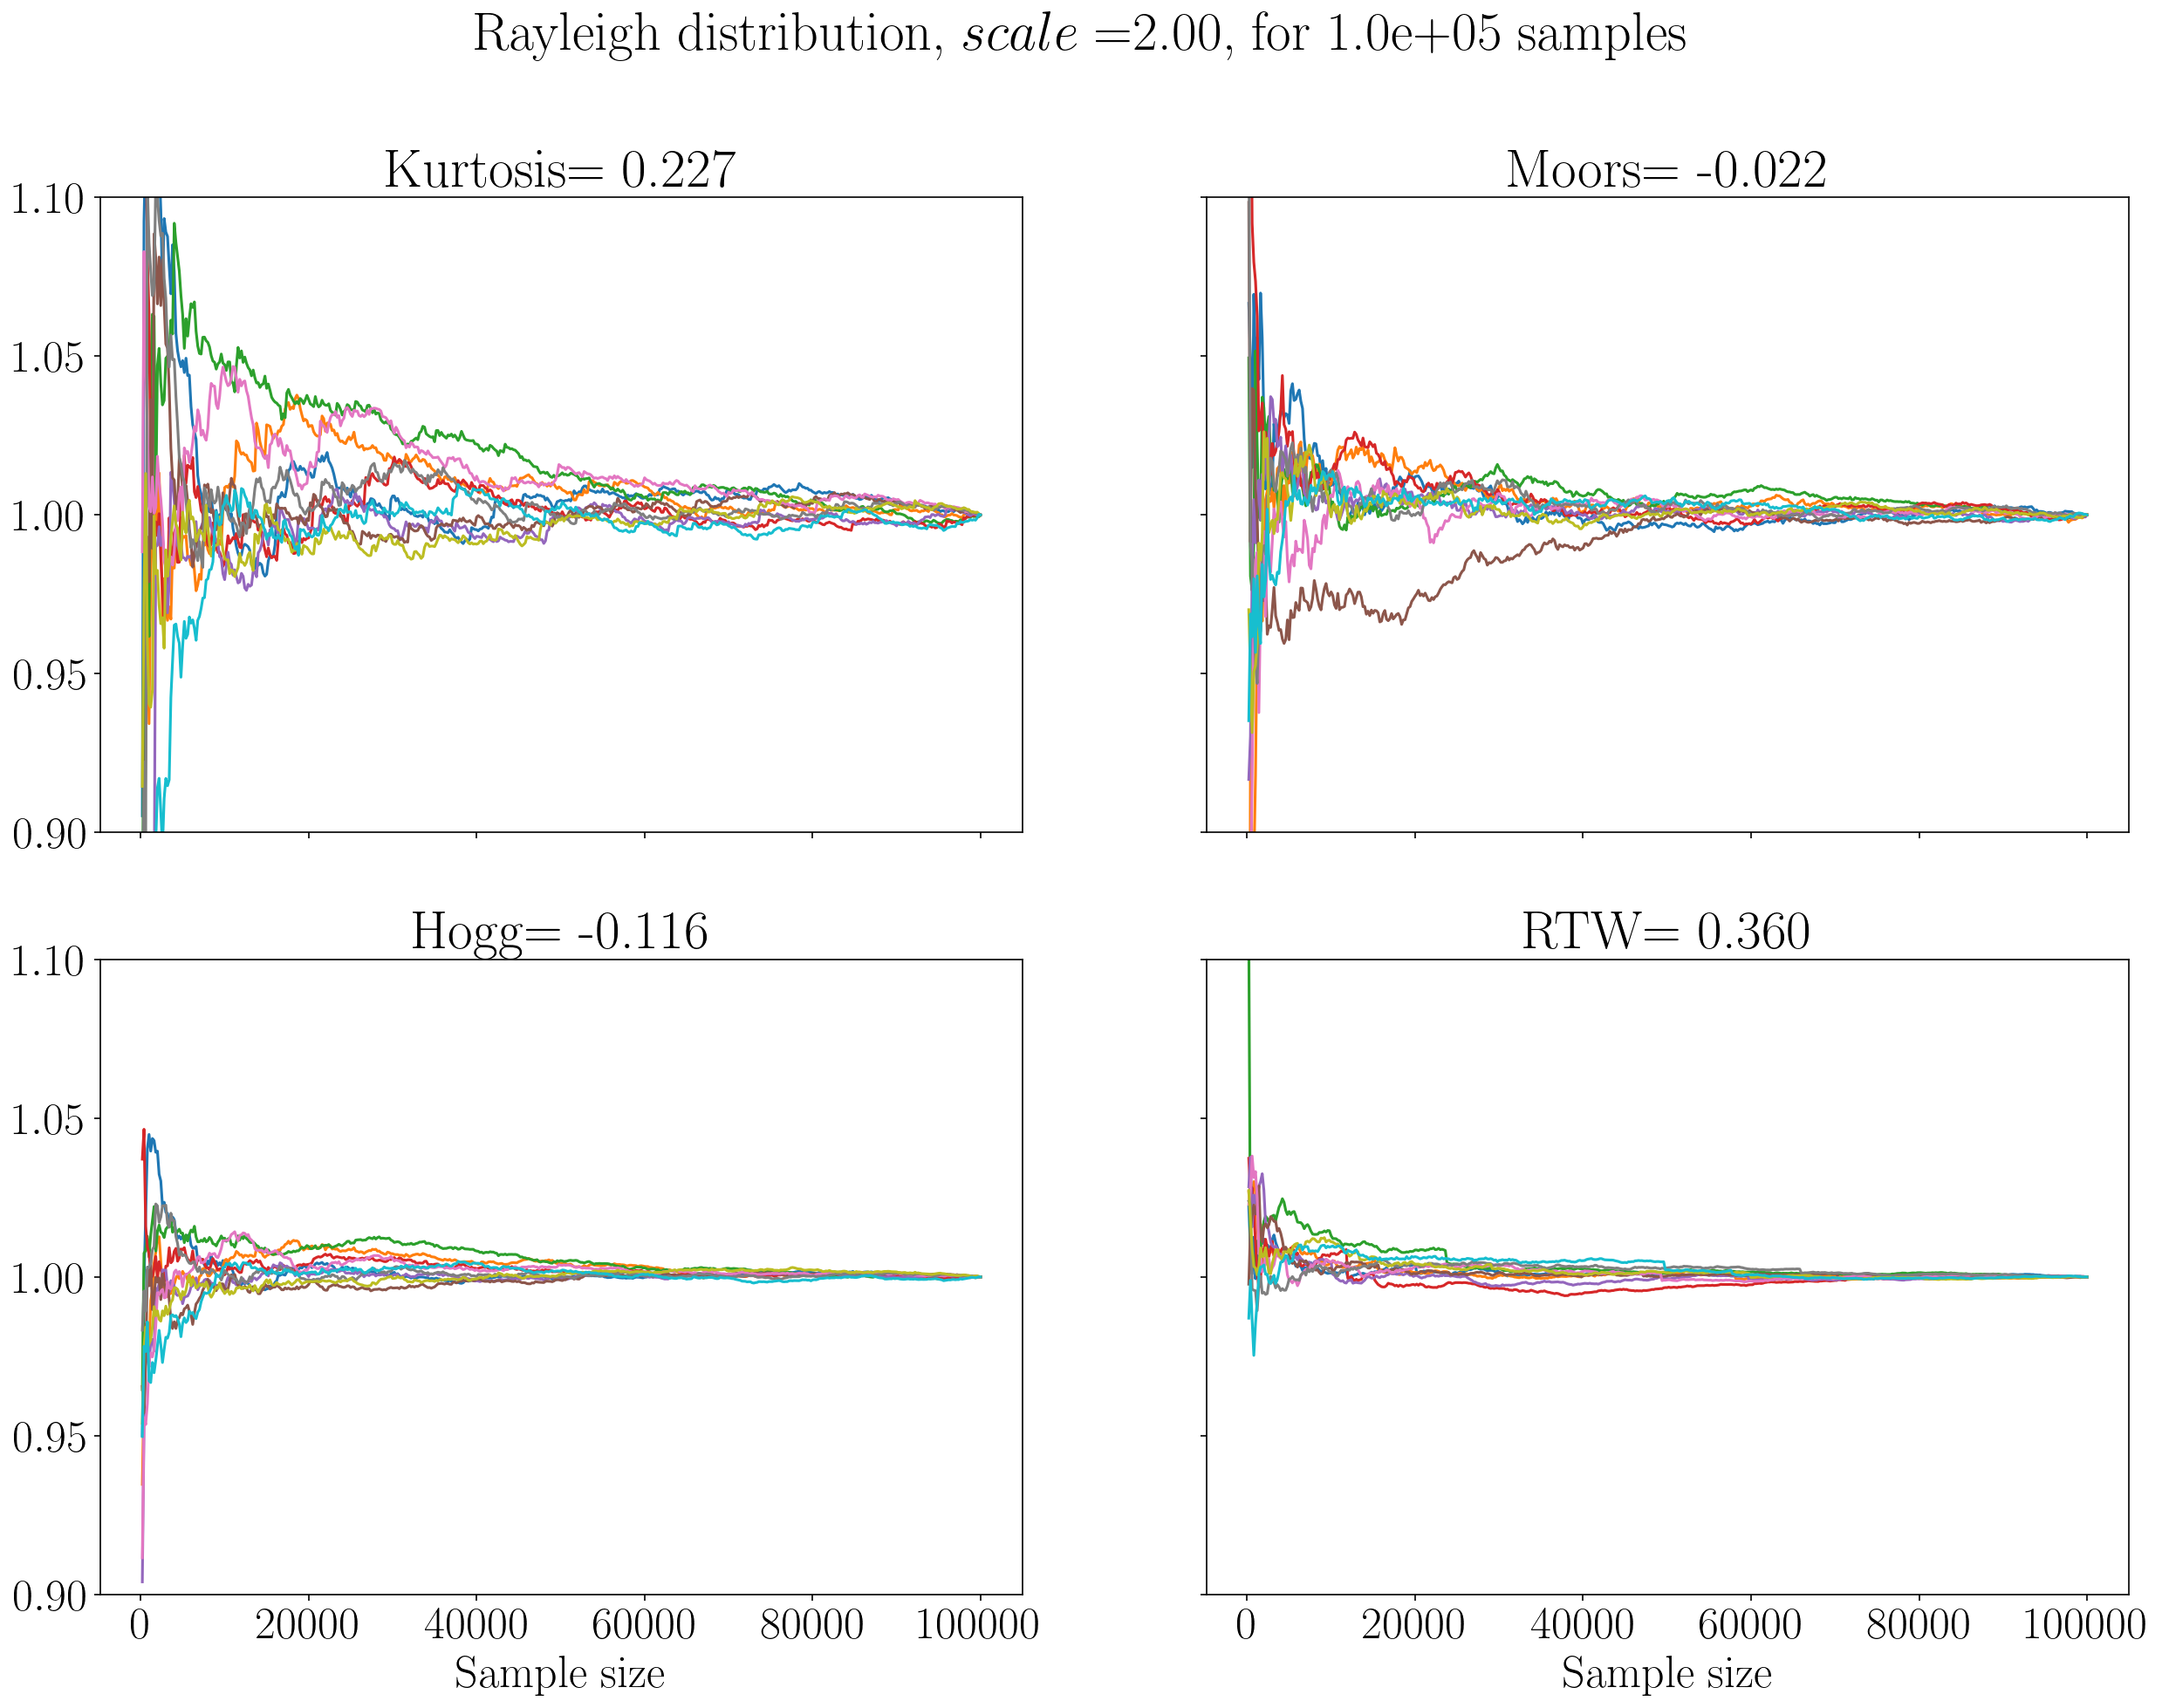
\includegraphics[width=\linewidth]{Images/Metrics/boot_rayleigh_convergence.png}
		\caption{ Evolution of the tail statistics: Kurtosis, Moors, Hogg and RTW calculated for a Rayleigh distribution of sample size $10^5$. 
		Each statistic is calculated every $200$ samples. After this is over for all the sample length, the original sample is scrambled and the same procedure is done. This is to show how fast this statistics converge and how much they might fluctuate due to an update of the sample. 
		Each statistic is calculated without correcting for the Gaussian value (ie. is calculated on  the kurtosis, not the excess kurtosis, etc.. ) and normalized to the final value. Only the title values are calculated corrected for the Gaussian values as defined above.	
		}
		\label{fig:convergence_1}
	\end{figure}
	
	Figure \ref{fig:convergence_1} shows this evolution for the excess kurtosis,the $Mo$, the $Hg$ and RTW metrics.
	This is done by taking an initial sample of a Rayleigh distribution of size $10^5$. 
	Each statistic is calculated every 200 samples, i.e for sample sizes $\left\lbrace 200, 400, 600, \dots, 10000\right\rbrace$, then the original sample is shuffled and the same procedure is done, and the shuffle is repeated 10 times.
	This means that, for each statistic, each shuffle converges to the same value since the final distribution is based on the same $10^5$ data points.  
	These statistics are calculated for their definitions without correcting to the Gaussian value and then normalized to the final value. 
	The values for the titles are calculated for the  $10^5$ data set on the excess definitions (corrected to the Gaussian values.)
	
	This displays of the robustness of these metrics, since we can see that the kurtosis is more affected by the update on the data, and even when sampled from the same parent distribution after 7000 (70\%) points, it still has fluctuations of about 2\%, while the other statistics show a better performance much earlier.	
	
	
	\subsection{Bootstrapping}
	\label{sec:EWS_boots}
	Given the sensible nature of metrics related to tail statistics, especially the kurtosis, 
	it is important to try to achieve a reliable result with the finite data-set we handle and, if possible, to give an estimate of the error when calculating such values. 
	
	For this purpose, we use a simple non-parametric bootstrapping method to calculate mean values and expected errors for the metrics, following  \cite{Wright2011}. 
	
	If $\Bar{x}$ is the data to be analyzed:
	\[
	\Bar{x}_0={x_0,x_1,\dots,x_n}
	\]
	the bootstrapping method consists of making new sample sets by randomly shuffling the data ${x_j}$ in the original sample, and applying the analysis to these new $\Bar{x}_k$ samples:
	
	\[
	\Bar{x}_k={x_{k_1},x_{k_2},\dots,x_{k_n}}
	\]
	
	Then, the average of the resulting analysis in all the samples, for a sufficiently large set of re-samples, converges to the real statistic. 
	In this way, we can get better confidence on our results, without taking new measurements.
	
	Since the resulting distribution of all the samples should converge to a normal distribution, this also gives us an estimate of the error of our result. 
	\footnote{In \cite{Wright2011} it is briefly mentioned that this does not always work well for kurtosis, but there is no a better method cited. Since kurtosis is really sensitive to outliers, the bootstrapping will oscillate  and an arbitrarily large set of re-samples might need to be made to have a clean normal distribution (this could be tested by fitting and the $\chi^2$?)}

	
	%\href{http://dx.doi.org/10.2139/ssrn.3360903 }{\underline{this paper} Davide talks about saddle point approximations and edgeworth series like better options } }}

\begin{figure}[H]
\centering
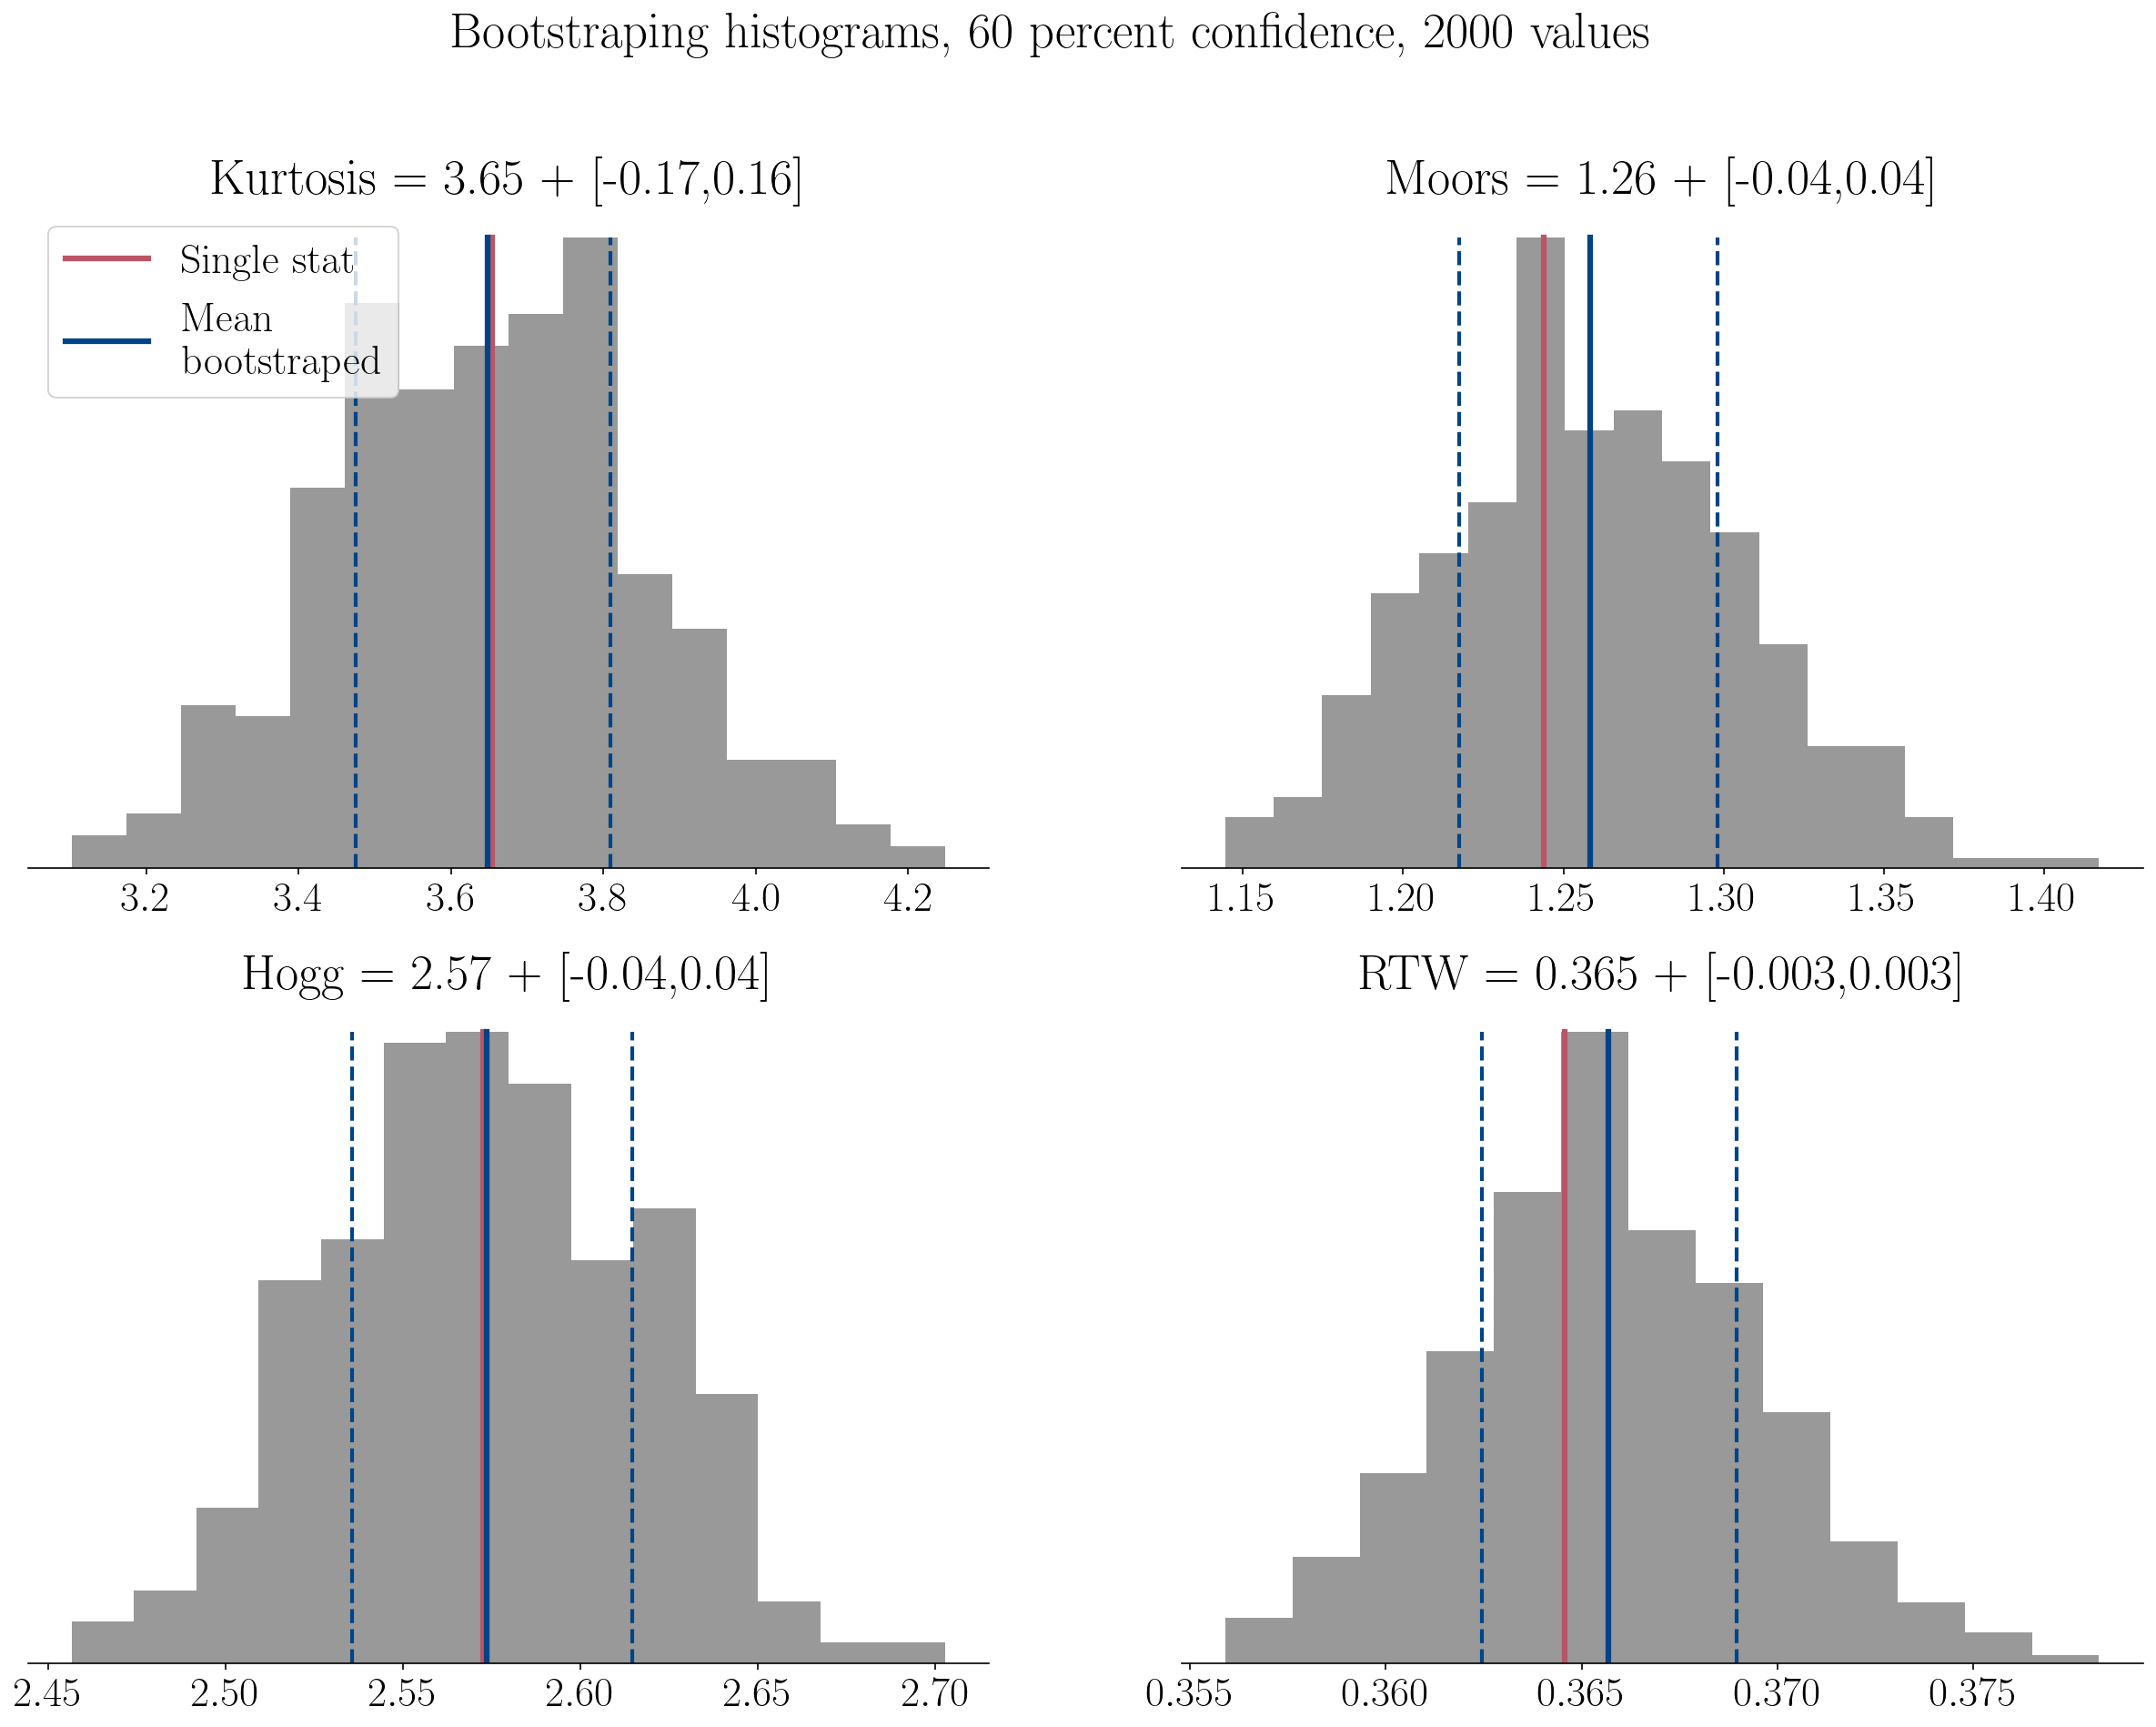
\includegraphics[width=\columnwidth]{Images/Metrics/boot_histograms_rayleigh_2000_400.png}
\caption{ Bootstrapping examples applied to a Rayleigh distribution with 2000 samples, after 400 resamples. The red line indicates the statistic calculated from bootstrapping, while the blue line is calculated from the samples, dashed blue indicate the 0.2 and 0.8 percentiles.  }
%	\caption{Events per ms}
\label{fig:Boots_example}
\end{figure}

In figure \ref{fig:Boots_example}  the result of applying the simple bootstrapping method to a sample of 2000 points from the Rayleigh distribution for 400 resamples is shown.
Each bootstrapping is done by resampling a data set of 70\% of the original data.
Applying this procedure for the Kurtosis,  $Hg$,  $Mo$ and  RTW yields Kurtosis$=3.65\pm 0.17$; $Hg=2.57\pm 0.04$, $Mo=1.26\pm 0.04$ and RTW=$0.365\pm 0.003$, where the errors are taken to have a $60\%$ confidence (0.2 and 0.8 percentiles) and the statistics are not corrected to the Gaussian values to better exemplify the relative error.

These results also show how more robust the RTW metrics are, since the relative errors after this particular bootstrapping are much lower than the relative error of the estimators and much lower than the relative error of the kurtosis.    

Appendix \ref{apx:boots} shows the same analysis for an exponential distribution to show the redundancy of the results.